\chapter{Semiclassical Dynamics of Bloch Electrons}
\label{ch:semiclassical}

The band structure of Chapter~\ref{ch:bloch} fixes the stationary states of an electron in a perfect crystal. This chapter asks how those electrons respond to applied fields. We build wavepackets out of Bloch states, state the semiclassical equations of motion, and apply them first to a static electric field (Bloch oscillations) and then to a magnetic field. There closed orbits on the Fermi surface are quantized into Landau levels, and the resulting quantum oscillations measure the Fermi surface directly.

% ============================================================
\section{Wave Packets of Bloch Electrons}
% ============================================================

In the semiclassical picture electrons do \emph{not} collide with the ions --- the mean free path is far too long for that --- but rather with imperfections in the crystal. To describe their response to applied fields we build wavepackets out of Bloch states.

\begin{definition}[Bloch wavepacket]
\begin{equation}
    \psi_n(\lvect{x},t) = \sum_{\lvect{k}'} g(\lvect{k}')\, \psi_{n\lvect{k}'}(\lvect{x})\, \exp\!\left(-\tfrac{i}{\hbar}\varepsilon_n(\lvect{k}')t\right),
\end{equation}
where the weight $g(\lvect{k}') \approx 0$ once $|\lvect{k}'-\lvect{k}| > \Delta k$. The packet must obey the uncertainty principle $\Delta k\, \Delta x \gtrsim 1$.
\end{definition}

\subsection{Width of the Wavepacket}

Assume $\Delta k$ is small compared with the dimensions of the Brillouin zone, and examine the amplitude at points a lattice vector away:
\begin{equation}
    \psi_n(\lvect{x}_0 + \cvect{R}, t) = \sum_{\lvect{k}'} \underbrace{\bigl[ g(\lvect{k}')\psi_{n\lvect{k}'}(\lvect{x}_0) \bigr]}_{\text{weight function}}
    \exp\!\left[ i\Bigl( \underbrace{\lvect{k}'\cdot\cvect{R}}_{\text{from the Bloch condition}} - \tfrac{1}{\hbar}\varepsilon_n(\lvect{k}')t \Bigr) \right].
\end{equation}
By the properties of the Fourier transform, if $g(\lvect{k})$ is appreciable within $\Delta k$ then $g(\lvect{x})$ is appreciable within $\Delta R \approx 1/\Delta k$. Since $\Delta k$ is small compared with the Brillouin zone dimension, of order $1/a$, the spread $\Delta R$ is large compared with the lattice constant $a$: wavepackets are spread over many primitive unit cells.

\subsection{Group Velocity of Bloch Electrons}

Expand the band energy to second order in a small shift $\lvect{q}$:
\begin{equation}
    \varepsilon_n(\lvect{k}+\lvect{q}) = \varepsilon_n(\lvect{k}) + \sum_i \pdv{\varepsilon_n}{k_i} q_i
    + \frac{1}{2}\sum_{ij} \frac{\partial^2 \varepsilon_n}{\partial k_i \partial k_j} q_i q_j + O(q^3).
    \label{eq:bloch-expand}
\end{equation}
The same shift can be treated by perturbation theory: since $H_{\lvect{k}+\lvect{q}}\psi^n_{\lvect{k}+\lvect{q}} = \varepsilon^n_{\lvect{k}+\lvect{q}}\psi^n_{\lvect{k}+\lvect{q}}$,
\begin{equation}
    H_{\lvect{k}+\lvect{q}} = H_{\lvect{k}} + \underbrace{\frac{\hbar^2}{m}\,\lvect{q}\cdot\left(\frac{1}{i}\nabla + \lvect{k}\right)}_{\displaystyle V(\lvect{q})} + \frac{\hbar^2}{2m}q^2 .
    \label{eq:bloch-Hexpand}
\end{equation}
If the unperturbed problem is $H_0 \psi_n = E^0_n \psi_n$, then to second order in $V$,
\begin{equation}
    E_n = E^0_n + \int d\lvect{x}\; \psi_n^* V \psi_n + \sum_{n' \neq n} \frac{\bigl| \int d\lvect{x}\; \psi_n^* V \psi_{n'} \bigr|^2}{E^0_n - E^0_{n'}}.
    \label{eq:bloch-pert}
\end{equation}
Comparing~\eqref{eq:bloch-expand} with~\eqref{eq:bloch-pert} at first order,
\begin{equation}
    \sum_i \pdv{\varepsilon_n}{k_i} q_i = \int d\lvect{x}\; \psi_n^* V \psi_n,
\end{equation}
and comparing~\eqref{eq:bloch-Hexpand} with~\eqref{eq:bloch-pert} we need the part of $V(\lvect{q})$ linear in $\lvect{q}$, so that
\begin{equation}
    \sum_i \pdv{\varepsilon_n}{k_i} q_i = \frac{\hbar^2}{m} \sum_i \int d\lvect{x}\; u^*_{n\lvect{k}}\, q_i \left(\frac{1}{i}\nabla + \lvect{k}\right)_{\!i} u_{n\lvect{k}}.
\end{equation}
Recalling the momentum operator $\hat{p}_i \equiv \frac{\hbar}{i}\pdv{}{x_i}$,
\begin{equation}
    \frac{1}{\hbar}\pdv{\varepsilon_n}{k_i} = \frac{1}{m} \Bigl\langle \frac{\hbar}{i}\pdv{}{x_i} + \hbar k_i \Bigr\rangle_{u_{n\lvect{k}}}
    = \frac{1}{m}\bigl\langle \hat{p}_i + \hbar k_i \bigr\rangle_{u_{n\lvect{k}}}.
\end{equation}
Finally, using $\psi_{n\lvect{k}} = e^{i\lvect{k}\cdot\lvect{x}} u_{n\lvect{k}}(\lvect{x})$,
\begin{equation}
    \frac{1}{\hbar}\pdv{\varepsilon_n}{k_i}
    = \frac{1}{m}\int d\lvect{x}\; u^*_{n\lvect{k}} (\hat{p}_i + \hbar k_i) u_{n\lvect{k}}
    = \frac{1}{m}\int d\lvect{x}\; e^{i\lvect{k}\cdot\lvect{x}} \psi^*_{n\lvect{k}} (\hat{p}_i + \hbar k_i) e^{-i\lvect{k}\cdot\lvect{x}} \psi_{n\lvect{k}},
\end{equation}
and since
\begin{equation}
    \hat{p}_i \bigl[ e^{-i\lvect{k}\cdot\lvect{x}} \psi_{n\lvect{k}}(\lvect{x}) \bigr]
    = \frac{\hbar}{i}\pdv{}{x_i}\bigl[ e^{-i\lvect{k}\cdot\lvect{x}} \psi_{n\lvect{k}}(\lvect{x}) \bigr]
    = -\hbar k_i\, e^{-i\lvect{k}\cdot\lvect{x}}\psi_{n\lvect{k}}(\lvect{x}) + e^{-i\lvect{k}\cdot\lvect{x}}\, \hat{p}_i \psi_{n\lvect{k}}(\lvect{x}),
\end{equation}
the $\hbar k_i$ terms cancel, leaving
\begin{equation}
    \frac{1}{\hbar}\pdv{\varepsilon_n}{k_i}
    = \frac{1}{m}\int d\lvect{x}\; e^{i\lvect{k}\cdot\lvect{x}} \psi^*_{n\lvect{k}} e^{-i\lvect{k}\cdot\lvect{x}} \hat{p}_i \psi_{n\lvect{k}}
    = \frac{1}{m}\langle \hat{p}_i \rangle_{\psi_{n\lvect{k}}} = \langle \hat{v}_i \rangle_{\psi_{n\lvect{k}}}.
\end{equation}

\begin{formula}[Group velocity]
\begin{equation}
    \langle \lvect{v}_n(\lvect{k}) \rangle = \frac{1}{\hbar} \pdv{\varepsilon_n(\lvect{k})}{\lvect{k}} = \pdv{\omega}{\lvect{k}}.
\end{equation}
\end{formula}

% ============================================================
\section{The Semiclassical Model}
\label{sec:bloch-semiclassical}
% ============================================================

The semiclassical model describes the response of electrons to externally applied electric and magnetic fields that vary slowly on the scale $\Delta R$ of the wavepacket. Given the band structure $\varepsilon_n(\lvect{k})$, it associates with each electron a position $\lvect{x}$, a wavevector $\lvect{k}$, and a band index $n$.

\begin{fact}[Assumptions of the semiclassical model]
\begin{enumerate}
    \item The electron stays within its band: there are no interband transitions.
    \item The time evolution is governed by
    \begin{equation}
        \dot{\lvect{x}} = \lvect{v}_n(\lvect{k}) = \frac{1}{\hbar}\pdv{\varepsilon_n(\lvect{k})}{\lvect{k}},
        \qquad
        \hbar \dot{\lvect{k}} = -e\left[ \cvect{E}(\lvect{x},t) + \frac{1}{c}\, \lvect{v}_n(\lvect{k}) \times \cvect{H}(\lvect{x},t) \right],
    \end{equation}
    where $\cvect{H}$ is the magnetic field. Note that the crystal momentum $\hbar\lvect{k}$ is \emph{not} the total electron momentum.
    \item All distinct wavevectors for a single band lie within a single primitive cell of the reciprocal lattice, with occupation given by the Fermi distribution
    \begin{equation}
        f\bigl(\varepsilon_n(\lvect{k})\bigr) \frac{d\lvect{k}}{4\pi^3}
        = \frac{d\lvect{k}/4\pi^3}{e^{(\varepsilon_n(\lvect{k})-\mu)/k_B T}+1}.
    \end{equation}
\end{enumerate}
\end{fact}

A useful corollary is the \emph{many-carrier} statement: one need only consider the types of carriers lying within $\sim k_B T$ of the Fermi level.

\subsection{Conditions of Validity}

There must be some minimum strength of the periodic potential below which the model breaks down, because interband transitions become possible. The conditions are
\begin{equation}
    e |\cvect{E}| a \ll \frac{\bigl[\varepsilon_{\text{gap}}(\lvect{k})\bigr]^2}{\varepsilon_F},
    \qquad
    \hbar\omega_c \ll \frac{\bigl[\varepsilon_{\text{gap}}(\lvect{k})\bigr]^2}{\varepsilon_F},
\end{equation}
where $\omega_c$ is the cyclotron frequency: both the work done by the field over a lattice constant and the cyclotron energy quantum must be small compared with the scale set by the gap.

\subsection{Bloch Oscillations}

Apply the model to an electron in a single band of a one-dimensional crystal of lattice constant $a$, in a uniform static field $E$ and no magnetic field. The Hamiltonian is
\begin{equation}
    H = \frac{p^2}{2m} + U(x) + eEx,
\end{equation}
and the equation of motion reduces to
\begin{equation}
    \hbar\dot{k} = -eE \qquad\Longrightarrow\qquad k(t) = k(0) - \frac{eEt}{\hbar}.
\end{equation}
The wavevector therefore moves uniformly through the Brillouin zone. On reaching one zone boundary it re-enters from the opposite one, since $k = \pm\pi/a$ label the same state: the one-dimensional Brillouin zone is topologically a circle. The velocity $v_n(k) = \hbar^{-1}\,\partial\varepsilon_n/\partial k$ is periodic in $k$ and changes sign across the zone, so the electron does not accelerate indefinitely but oscillates.

\begin{formula}[Bloch oscillation period]
\begin{equation}
    T_B = \frac{2\pi\hbar}{eEa}, \qquad \nu_B = \frac{eEa}{h}.
\end{equation}
\end{formula}

Integrating the velocity shows the real-space motion is bounded as well. For a tight-binding $s$-band $\varepsilon(k) = -2\gamma\cos ka$,
\begin{equation}
    x(t)-x(0) = \frac{1}{\hbar}\int_0^t \pdv{\varepsilon}{k}\,dt'
    = \frac{\varepsilon\bigl(k(t)\bigr) - \varepsilon\bigl(k(0)\bigr)}{-eE},
\end{equation}
so the amplitude of the oscillation is the bandwidth divided by the force, $4\gamma/eE$.

\begin{fact}[Consequences of Bloch oscillations]
\begin{enumerate}
    \item A \emph{static} electric field produces an \emph{oscillating} current: a perfect crystal would act as a DC-to-AC converter.
    \item In real solids the oscillations are almost never seen, because the scattering time from impurities and phonons is much shorter than $T_B$. They have been observed directly with cold atoms in optical lattices, and in semiconductor superlattices, where the large period $a$ shortens $T_B$.
    \item At strong fields the electron can tunnel into a higher band instead of Bragg reflecting. This \emph{Zener tunnelling} is exactly the interband transition excluded by the validity condition on $e|\cvect{E}|a$ above.
\end{enumerate}
\end{fact}

% ============================================================
\section{Semiclassical Motion in a Magnetic Field}
\label{sec:bloch-magnetic}
% ============================================================

This section and the next two are written in SI units. The carrier charge is $q$, with $q = -e$ for an electron, and the semiclassical equations of Section~\ref{sec:bloch-semiclassical} read
\begin{equation}
    \dot{\lvect{r}} = \lvect{v}(\lvect{k}) = \frac{1}{\hbar}\nabla_{\lvect{k}}\varepsilon_n(\lvect{k}),
    \qquad
    \hbar\dot{\lvect{k}} = q\bigl(\cvect{E} + \dot{\lvect{r}}\times\cvect{B}\bigr).
\end{equation}
In Gaussian units, replace $\hbar/(eB)\to\hbar c/(eB)$ and $\Phi_0 = 2\pi\hbar c/e$.

\begin{definition}[Magnetic length]
\begin{equation}
    \ell = \sqrt{\frac{\hbar}{|q|B}} \approx \frac{25.7\ \text{nm}}{\sqrt{B/\text{T}}}.
\end{equation}
Below, $A_k$ denotes an area in $k$-space (units m$^{-2}$) and $A_r$ an area in real space (units m$^2$).
\end{definition}

\begin{fact}[$B$ or $H$?]
The Lorentz force involves $\cvect{B}$, the field inside the sample, so all equations of motion and quantization conditions are written in terms of $B$. Ashcroft and Mermin write $H$, because in Gaussian units $B = H$ in vacuum and $H$ is what the experimenter applies; the two differ by $\cvect{B} = \cvect{H} + 4\pi\cvect{M}$. For a non-magnetic metal $\chi\sim10^{-5}$, so $B\approx H$. The distinction matters only when the oscillating magnetization becomes large (very pure samples at low $T$). The electrons then feel a field that depends on the magnetization they produce, which distorts the waveform and generates harmonics (the \emph{Shoenberg effect}, or magnetic interaction). Strictly, quantum oscillations are periodic in $1/B$.
\end{fact}

\subsection{Conserved Quantities}

With $\cvect{E} = 0$ two quantities are conserved.
\begin{itemize}
    \item \emph{Energy:} the force is perpendicular to the velocity, which is the $k$-gradient of the energy, so $d\varepsilon/dt = \nabla_{\lvect{k}}\varepsilon\cdot\dot{\lvect{k}} \propto \lvect{v}\cdot(\lvect{v}\times\cvect{B}) = 0$.
    \item \emph{Wavevector along the field:} $\hbar\dot{\lvect{k}}\perp\cvect{B}$, so $k_\parallel = \uvect{B}\cdot\lvect{k}$ is constant.
\end{itemize}
In $k$-space an electron therefore moves along the intersection of a constant-energy surface with a plane perpendicular to $\cvect{B}$. At the Fermi energy these curves are slices of the Fermi surface.

Take $\cvect{B} = B\uvect{z}$, so the conserved component is $k_z$. An orbit lies in a plane perpendicular to $\cvect{B}$, with $k_z$ labelling which plane, so every closed orbit is specified by two numbers, and so is the $k$-space area it encloses: $A_k = A_k(\varepsilon, k_z)$. Changing either one changes the area,
\begin{equation}
    dA_k = \left.\pdv{A_k}{\varepsilon}\right|_{k_z}d\varepsilon + \left.\pdv{A_k}{k_z}\right|_{\varepsilon}dk_z.
    \label{eq:semi-dA}
\end{equation}
The first term describes the orbit growing within one plane as the energy rises. The second describes moving between planes along the Fermi surface. The cyclotron mass turns out to be controlled entirely by the first, because a single electron never leaves its plane.

\begin{definition}[Closed and open orbits]
If the slice is a closed curve, the orbit is \emph{closed}, and periodic in time. If the Fermi surface is open and the slice runs through the zone boundary without closing, the orbit is \emph{open}: extended and aperiodic in real space along one direction.
\end{definition}

Closed orbits give a magnetoresistance that saturates at high field. Open orbits give a magnetoresistance that does not saturate, which produces sharp features in the resistance as the field direction is rotated. Only closed orbits are Landau-quantized, and everything below concerns closed orbits.

\subsection{Real-Space Orbits}

Integrate $\hbar\dot{\lvect{k}} = q\,\dot{\lvect{r}}\times\cvect{B}$ in time at constant $\cvect{B}$:
\begin{equation}
    \hbar\,\Delta\lvect{k} = q\,\Delta\lvect{r}\times\cvect{B}.
\end{equation}
Only the part of $\Delta\lvect{r}$ perpendicular to $\cvect{B}$ survives on the right. Define $\lvect{r}_\perp = \lvect{r} - (\uvect{B}\cdot\lvect{r})\uvect{B}$, cross with $\uvect{B}$ from the left, and use $\uvect{B}\times(\Delta\lvect{r}\times\cvect{B}) = B\,\Delta\lvect{r}_\perp$.

\begin{formula}[Real-space orbit]
\begin{equation}
    \Delta\lvect{r}_\perp = \frac{\hbar}{qB}\,\uvect{B}\times\Delta\lvect{k}
    \qquad\xrightarrow{\;q=-e\;}\qquad
    \Delta\lvect{r}_\perp = -\ell^2\,\uvect{B}\times\Delta\lvect{k}.
\end{equation}
The real-space orbit is the $k$-space orbit \textbf{rotated by $90^\circ$} about $\cvect{B}$, in a sense set by the sign of $q$, and \textbf{scaled by $\ell^2 = \hbar/(|q|B)$}. Areas therefore scale by $\ell^4$:
\begin{equation}
    A_r = \ell^4A_k = \left(\frac{\hbar}{eB}\right)^2A_k.
\end{equation}
\end{formula}

\begin{figure}[ht]
\centering
\begin{tikzpicture}[scale=0.9,>=Stealth]
  \begin{scope}
    \draw[->,gray] (-2,0)--(2,0) node[right]{$k_x$};
    \draw[->,gray] (0,-1.6)--(0,1.8) node[above]{$k_y$};
    \draw[thick,blue!60!black,
      postaction={decorate,decoration={markings,mark=at position 0.15 with {\arrow{>}},
                  mark=at position 0.65 with {\arrow{>}}}}]
      plot[smooth cycle] coordinates {(1.5,0) (0.8,0.9) (-0.6,1.0) (-1.4,0.2) (-0.9,-0.9) (0.6,-1.0)};
    \node at (0,-2.1) {$k$-space orbit (slice of FS)};
  \end{scope}
  \draw[->,thick] (2.6,0) -- node[above]{rotate $90^\circ$} node[below]{scale by $\ell^2$} (5.0,0);
  \begin{scope}[shift={(7.6,0)}]
    \draw[->,gray] (-2,0)--(2,0) node[right]{$x$};
    \draw[->,gray] (0,-1.8)--(0,2) node[above]{$y$};
    \draw[thick,red!60!black,
      postaction={decorate,decoration={markings,mark=at position 0.15 with {\arrow{>}},
                  mark=at position 0.65 with {\arrow{>}}}}]
      plot[smooth cycle] coordinates {(0,1.5) (-0.9,0.8) (-1.0,-0.6) (-0.2,-1.4) (0.9,-0.9) (1.0,0.6)};
    \node at (0,-2.3) {real-space orbit};
  \end{scope}
\end{tikzpicture}
\caption{The real-space orbit is the $k$-space orbit rotated by $90^\circ$ about $\cvect{B}$ and scaled by $\ell^2$.}
\label{fig:bloch-real-orbit}
\end{figure}

\begin{example}[Size of a cyclotron orbit]
At $B = 10$\,T, $\ell\approx8$\,nm. With $k_F\sim10^{10}$\,m$^{-1}$, the cyclotron radius is $r_c = \ell^2k_F\approx0.7\ \mu$m. That is thousands of lattice spacings, which justifies the semiclassical wavepacket picture.
\end{example}

\subsection{Cyclotron Period and Cyclotron Mass}

The cross product in the equation of motion discards the component of $\lvect{v}$ along $\cvect{B}$. Only the in-plane part
\begin{equation}
    \lvect{v}_\perp = (v_x, v_y) = \frac{1}{\hbar}\nabla_\perp\varepsilon,
    \qquad
    \nabla_\perp\varepsilon \equiv \left(\pdv{\varepsilon}{k_x}, \pdv{\varepsilon}{k_y}\right),
\end{equation}
drives the motion around the orbit, with $|\lvect{v}\times\cvect{B}| = v_\perp B$ and so $|\dot{\lvect{k}}| = |q|Bv_\perp/\hbar$. Within the plane, $\lvect{v}_\perp$ points along the normal to the orbit: $\varepsilon$ does not change along the orbit, so its in-plane gradient has no tangential component. The electron moves \emph{along} the orbit in $k$-space while its in-plane velocity points \emph{across} it. If $dk$ is an element of arc length along the orbit, the time spent on it is $dt = dk/|\dot{\lvect{k}}|$, and the period is
\begin{equation}
    T = \oint\frac{dk}{|\dot{\lvect{k}}|} = \frac{\hbar}{|q|B}\oint\frac{dk}{v_\perp}.
    \label{eq:semi-T-loop}
\end{equation}
The electron lingers where $v_\perp$ is small, that is, where the band is flat within the plane.

Now hold $k_z$ fixed and compare the orbits at $\varepsilon$ and $\varepsilon + d\varepsilon$. From a point $\lvect{k}$ on the inner orbit, step a distance $\delta k$ along the in-plane normal $\uvect{n} = \nabla_\perp\varepsilon/|\nabla_\perp\varepsilon|$. Taylor expanding, $\varepsilon(\lvect{k} + \delta k\,\uvect{n}) \approx \varepsilon(\lvect{k}) + |\nabla_\perp\varepsilon|\,\delta k$. Landing on the outer orbit means this equals $\varepsilon + d\varepsilon$, so the local spacing between neighbouring orbits is
\begin{equation}
    \delta k = \frac{d\varepsilon}{|\nabla_\perp\varepsilon|} = \frac{d\varepsilon}{\hbar v_\perp},
\end{equation}
the two-dimensional version of $dx = df/f'(x)$. Like contour lines on a map, neighbouring orbits are close together where the energy changes steeply and far apart where it changes slowly.

Only the in-plane gradient appears because the step stays in the plane, so $\partial\varepsilon/\partial k_z = \hbar v_z$ never contributes. Geometrically, the surfaces at $\varepsilon$ and $\varepsilon + d\varepsilon$ bound a thin shell of thickness $d\varepsilon/(\hbar|\lvect{v}|)$. A plane of fixed $k_z$ generally cuts this shell at an angle (think of an off-centre slice through a thin spherical shell), so the annulus it leaves is wider than the shell is thick: $\delta k = d\varepsilon/(\hbar v_\perp) \ge d\varepsilon/(\hbar|\lvect{v}|)$.

\begin{figure}[ht]
\centering
\begin{tikzpicture}[scale=1.15,>=Stealth]
  \def\outer{plot[smooth cycle] coordinates {(2.05,0) (1.15,1.25) (-0.55,1.3) (-1.75,0.35) (-1.3,-1.0) (0.6,-1.25)}}
  \def\inner{plot[smooth cycle] coordinates {(1.6,0) (0.9,0.95) (-0.5,1.05) (-1.5,0.3) (-1.1,-0.85) (0.5,-1.0)}}
  \fill[orange!30] \outer;
  \fill[white] \inner;
  \draw[thick,red!60!black] \outer;
  \draw[thick,blue!60!black] \inner;
  \draw[->,thick] (1.6,0) -- (2.05,0);
  \node[right] at (2.1,0) {$\delta k=\dfrac{d\varepsilon}{\hbar v_\perp}$};
  \node at (0,0) {$\varepsilon$};
  \node[red!60!black] at (1.9,1.3) {$\varepsilon+d\varepsilon$};
\end{tikzpicture}
\caption{Neighbouring orbits at fixed $k_z$. The shaded strip between them has area $dA_k = \oint\delta k\,dk$.}
\label{fig:semi-strip}
\end{figure}

An arc element $dk$ of the inner orbit contributes an area $\delta k\,dk$ to the strip between the two orbits (Figure~\ref{fig:semi-strip}). Summing around the loop,
\begin{equation}
    dA_k = \oint\delta k\,dk = d\varepsilon\oint\frac{dk}{\hbar v_\perp}
    \qquad\Longrightarrow\qquad
    \left.\pdv{A_k}{\varepsilon}\right|_{k_z} = \oint\frac{dk}{\hbar v_\perp}.
    \label{eq:semi-dAde}
\end{equation}

The loop integrals in~\eqref{eq:semi-T-loop} and~\eqref{eq:semi-dAde} are identical up to a factor of $\hbar$. This is not a coincidence: the same in-plane velocity sets both how fast the electron moves around the orbit and how far apart neighbouring orbits are. Substituting, and defining the cyclotron mass through the free-electron form $\omega_c = |q|B/m^*$:

\begin{formula}[Cyclotron frequency for an arbitrary closed orbit]
\begin{equation}
    T = \frac{\hbar^2}{|q|B}\left.\pdv{A_k}{\varepsilon}\right|_{k_z},
    \qquad
    \omega_c = \frac{2\pi}{T} = \frac{|q|B}{m^*},
    \qquad
    m^* \equiv \frac{\hbar^2}{2\pi}\left.\pdv{A_k(\varepsilon,k_z)}{\varepsilon}\right|_{k_z}.
\end{equation}
\end{formula}

For free electrons the orbit is a circle with $\hbar v_\perp = \hbar^2k/m$ everywhere, so $\oint dk/(\hbar v_\perp) = 2\pi m/\hbar^2 = d(\pi k^2)/d\varepsilon$, and $m^* = m$. In general $m^*$ is a property of a whole orbit, not of a point in $k$-space: it measures how fast the orbit area grows with energy, and it depends on $\varepsilon$, on $k_z$, and on the direction of $\cvect{B}$ (which sets the family of planes). The derivative is taken at fixed $k_z$ because the period refers to one orbit, and one orbit stays in one plane. Comparing orbits on different planes would bring in the second term of~\eqref{eq:semi-dA}, a change of area from sliding along the Fermi surface that has nothing to do with how long the electron takes to go around.

% ============================================================
\section{Onsager Quantization and Landau Levels}
\label{sec:bloch-onsager}
% ============================================================

\subsection{Bohr--Sommerfeld Quantization}

A closed orbit is periodic, so the electron's wavefunction must return to itself after one loop. The total phase it accumulates must be a whole multiple of $2\pi$, up to a fixed correction:
\begin{equation}
    \Delta\varphi_{\text{loop}} = 2\pi(n+\gamma), \qquad n = 0,1,2,\ldots
\end{equation}
For an ordinary orbit $\gamma = \tfrac12$. This is the same $\tfrac12$ as in the harmonic-oscillator energies $\hbar\omega(n+\tfrac12)$, and it comes from the points where the semiclassical approximation breaks down along the orbit. $\gamma$ sets the \emph{phase} of the quantum oscillations, not their period. In systems with a Berry phase $\phi_B$, such as graphene, $\gamma = \tfrac12 - \phi_B/2\pi$.

The phase is accumulated by the \emph{canonical} momentum $\lvect{p}_c = -i\hbar\nabla$, which measures how fast the phase of the wavefunction changes in space. In the Hamiltonian it is the momentum inside the parentheses, not the kinetic momentum:
\begin{equation}
    H = \frac{1}{2m}\bigl(\lvect{p}_c - q\cvect{A}\bigr)^2,
    \qquad
    m\lvect{v} = \lvect{p}_c - q\cvect{A} \;\longleftrightarrow\; \hbar\lvect{k}.
\end{equation}

\begin{formula}[Bohr--Sommerfeld condition]
\begin{equation}
    \oint\lvect{p}_c\cdot d\lvect{r} = 2\pi\hbar(n+\gamma),
    \qquad
    \lvect{p}_c = \hbar\lvect{k} + q\cvect{A}.
\end{equation}
\end{formula}

$\lvect{p}_c$ itself is gauge-dependent, but its loop integral is gauge-invariant, because the $\cvect{A}$ part becomes a magnetic flux (the Aharonov--Bohm phase).

\subsection{The Onsager Relation}

Split the loop integral into its two pieces. By Stokes' theorem the vector-potential term is
\begin{equation}
    q\oint\cvect{A}\cdot d\lvect{r} = q\int(\nabla\times\cvect{A})\cdot d\lvect{s} = q\,\cvect{B}\cdot\uvect{n}\,A_r \equiv q\Phi,
\end{equation}
where $\Phi$ is the flux through the real-space orbit, oriented by the direction of travel. For the kinetic term, integrating the equation of motion gives $\hbar\lvect{k} = q\,\lvect{r}\times\cvect{B} + \text{const}$. The constant integrates to zero around a closed loop, and with $\oint\lvect{r}\times d\lvect{r} = 2A_r\uvect{n}$,
\begin{equation}
    \oint\hbar\lvect{k}\cdot d\lvect{r} = q\oint(\lvect{r}\times\cvect{B})\cdot d\lvect{r} = -q\,\cvect{B}\cdot\oint\lvect{r}\times d\lvect{r} = -2q\Phi.
\end{equation}
The kinetic term is twice the vector-potential term, and opposite in sign:
\begin{equation}
    \oint\lvect{p}_c\cdot d\lvect{r} = -2q\Phi + q\Phi = -q\Phi = 2\pi\hbar(n+\gamma).
\end{equation}

\begin{theorem}[Flux quantization and the Onsager relation]
The flux through an allowed orbit is a whole number of flux quanta, shifted by $\gamma$ (half-integer when $\gamma = \tfrac12$):
\begin{equation}
    |\Phi_n| = BA_r = (n+\gamma)\Phi_0,
    \qquad
    \Phi_0 = \frac{h}{e} = \frac{2\pi\hbar}{e}\approx4.14\times10^{-15}\ \text{T\,m}^2.
\end{equation}
Using $A_r = \ell^4A_k$, the allowed $k$-space areas are
\begin{equation}
    A_k(\varepsilon_n) = 2\pi(n+\gamma)\frac{eB}{\hbar} = \frac{2\pi(n+\gamma)}{\ell^2}.
\end{equation}
Nothing here depends on the shape of the band: \emph{any} closed orbit in \emph{any} Bloch band is quantized this way. The Landau levels are the energies whose constant-energy contours enclose exactly these areas.
\end{theorem}

\subsection{Check: Free-Electron Landau Levels}

In the Landau gauge $\cvect{A} = (0, Bx, 0)$, try $\psi(x,y) = e^{iky}f_k(x)$:
\begin{equation}
    \varepsilon f_k(x) = \frac{1}{2m}\left[-\hbar^2\frac{d^2}{dx^2} + (eB)^2(x-x_0)^2\right]f_k(x),
    \qquad
    x_0 = \frac{\hbar k}{eB} = k\ell^2.
\end{equation}
This is a one-dimensional harmonic oscillator centred at $x_0$ with frequency $\omega_c = eB/m$, so $\varepsilon_n = \hbar\omega_c(n+\tfrac12)$, independent of $k$: each level is highly degenerate.

From Onsager instead: for $\varepsilon = \hbar^2k^2/2m$, $A_k(\varepsilon) = 2\pi m\varepsilon/\hbar^2$, and setting this equal to $2\pi(n+\gamma)eB/\hbar$ gives
\begin{equation}
    \varepsilon_n = \frac{\hbar eB}{m}(n+\gamma) = \hbar\omega_c\bigl(n+\tfrac12\bigr)\quad(\gamma = \tfrac12),
\end{equation}
in exact agreement.

\begin{formula}[Landau-level spacing in a general band]
\begin{equation}
    \Delta\varepsilon = \frac{\Delta A_k}{\partial A_k/\partial\varepsilon}
    = \frac{2\pi eB/\hbar}{2\pi m^*/\hbar^2} = \hbar\frac{eB}{m^*} = \hbar\omega_c,
\end{equation}
with the cyclotron mass $m^*$ of Section~\ref{sec:bloch-magnetic}.
\end{formula}

\subsection{Landau-Level Degeneracy}

In the Landau gauge, periodic boundary conditions in $y$ give $k = 2\pi m/L_y$. The orbit centre must lie inside the sample, $0 < x_0 = k\ell^2 < L_x$, so $0 < m < L_xL_y/(2\pi\ell^2)$.

The same count follows from Onsager for any band. When $B$ is turned on, the uniform grid of allowed $k$-points (density $\text{Area}/(2\pi)^2$) collapses onto the quantized rings. Each ring collects the states from the annulus between neighbouring orbits, whose area is $\Delta A_k = A_k(n+1) - A_k(n) = 2\pi/\ell^2$. The number of states per level is therefore
\begin{equation}
    N = \text{Area}\int_{\text{annulus}}\frac{d^2k}{(2\pi)^2} = \frac{\text{Area}}{(2\pi)^2}\cdot\frac{2\pi}{\ell^2}.
\end{equation}

\begin{formula}[Landau-level degeneracy]
\begin{equation}
    N = \frac{\text{Area}}{2\pi\ell^2} = \frac{B\cdot\text{Area}}{\Phi_0}\qquad\text{(per spin)}:
\end{equation}
one state per flux quantum threading the sample. The degeneracy is the same for Bloch electrons in any band, because it depends only on the area between neighbouring orbits, which Onsager fixes independently of the band.
\end{formula}

\begin{figure}[ht]
\centering
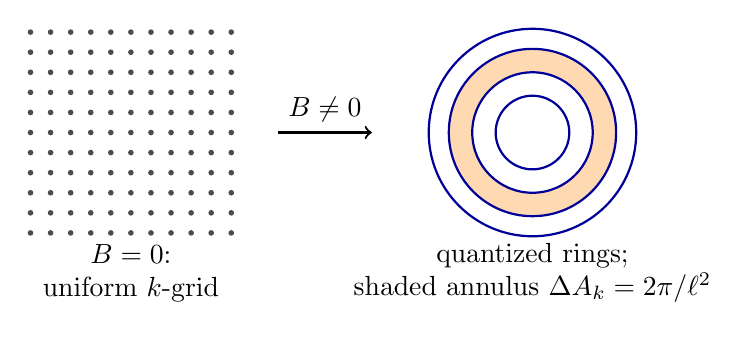
\begin{tikzpicture}[scale=0.85]
  \foreach \i in {-5,...,5}{\foreach \j in {-5,...,5}{\fill[black!70] (0.3*\i,0.3*\j) circle (1.2pt);}}
  \node[align=center] at (0,-2.1) {$B=0$:\\ uniform $k$-grid};
  \draw[->,thick] (2.2,0)--(3.6,0) node[midway,above]{$B\neq0$};
  \begin{scope}[shift={(6.0,0)}]
    \fill[orange!30] (0,0) circle (1.25); \fill[white] (0,0) circle (0.9);
    \foreach \r in {0.55,0.9,1.25,1.55}{\draw[thick,blue!60!black] (0,0) circle (\r);}
    \node[align=center] at (0,-2.1) {quantized rings;\\ shaded annulus $\Delta A_k=2\pi/\ell^2$};
  \end{scope}
\end{tikzpicture}
\caption{A magnetic field collapses the uniform grid of $k$-points onto the Landau rings. Each ring collects the states of one annulus of area $2\pi/\ell^2$.}
\label{fig:bloch-landau-rings}
\end{figure}

$\ell$ is \emph{not} the size of a classical orbit: in a metal $r_c = \ell^2k_F\gg\ell$. It is better thought of as the mean spacing between orbit centres of the same level, which are packed with one centre per area $2\pi\ell^2$.

% ============================================================
\section{Quantum Oscillations}
\label{sec:bloch-dhva}
% ============================================================

\subsection{Why Periodic in $1/B$}

As $B$ increases, every Landau level's area $2\pi(n+\gamma)eB/\hbar$ grows, so the levels move up in energy, and their degeneracy grows. With the electron number fixed, the highest occupied level empties out and crosses the Fermi energy, and the chemical potential jumps down to the next level, giving a sawtooth in $\mu(B)$. Each crossing produces a feature in every thermodynamic and transport quantity.

Level $n$ crosses $\varepsilon_F$ when its quantized area equals the Fermi-surface cross-section $A_F$:
\begin{equation}
    A_F = 2\pi(n+\gamma)\frac{eB_n}{\hbar}
    \qquad\Longrightarrow\qquad
    \frac{1}{B_n} = \frac{2\pi e}{\hbar A_F}(n+\gamma).
\end{equation}
Consecutive crossings are therefore evenly spaced in $1/B$.

\begin{formula}[de Haas--van Alphen period and frequency]
\begin{equation}
    \Delta\!\left(\frac1B\right) = \frac{1}{B_{n+1}} - \frac{1}{B_n} = \frac{2\pi e}{\hbar A_F},
    \qquad
    F \equiv \frac{1}{\Delta(1/B)} = \frac{\hbar}{2\pi e}A_F.
\end{equation}
In Gaussian units, $\Delta(1/B) = 2\pi e/(\hbar cS_F)$. The frequency $F$ (in tesla) measures the extremal Fermi-surface cross-section directly.
\end{formula}

\begin{example}[Order of magnitude]
For $k_F = 10^{10}$\,m$^{-1}$, $A_F = \pi k_F^2\approx3\times10^{20}$\,m$^{-2}$ and $F\approx3\times10^4$\,T, so $\Delta(1/B)\approx3\times10^{-5}$\,T$^{-1}$. At $10$\,T thousands of levels are occupied, and the oscillations are rapid in $B$.
\end{example}

The oscillating part of the susceptibility (de Haas--van Alphen) or of the resistivity (Shubnikov--de Haas) contains harmonics $p$,
\begin{equation}
    \chi_{\text{osc}} \sim \sum_p A_p\cos\!\left[2\pi p\left(\frac{F}{B}-\gamma\right) + \phi_p\right].
\end{equation}
It is periodic in $1/B$, so plotted against $B$ the oscillations get faster at low field.

\subsection{Extremal Orbits in Three Dimensions}

In three dimensions $k_z$ (along $\cvect{B}$) is conserved, and each slice has its own area $A(k_z)$. The total response sums the contributions of all slices:
\begin{equation}
    \chi_{\text{osc}} \sim \int dk_z\,\exp\!\left[\frac{i\hbar}{eB}A(k_z)\right] + \text{c.c.}
\end{equation}
Because $\hbar A/(eB)$ is huge, the phase varies rapidly with $k_z$ and the contributions cancel, \emph{except} near the values of $k_z$ where $A(k_z)$ is stationary.

\begin{fact}[Extremal cross-sections]
Only cross-sections with $\partial A/\partial k_z = 0$ contribute. Each extremal orbit (a maximum or minimum of $A(k_z)$) contributes one frequency $F_i = \hbar A_{\text{ext},i}/(2\pi e)$. Several extremal orbits give several frequencies, and their superposition produces \emph{beating}. Rotating $\cvect{B}$ and tracking $F(\theta)$ maps out the Fermi surface.
\end{fact}

The extremal plane $k_z^{\text{ext}}(\varepsilon)$ shifts slightly as the energy changes, so following the extremal area from $\varepsilon$ to $\varepsilon+d\varepsilon$ really does compare orbits on different planes. But by~\eqref{eq:semi-dA} the extra term is proportional to $\partial A_k/\partial k_z$, which vanishes there. To first order, $dA_{\text{ext}}/d\varepsilon = \partial A_k/\partial\varepsilon|_{k_z^{\text{ext}}}$, so the cyclotron mass of an extremal orbit is unambiguous.

\begin{formula}[Cyclotron mass of an extremal orbit]
\begin{equation}
    m^* = \frac{\hbar^2}{2\pi}\left.\frac{dA_{\text{ext}}}{d\varepsilon}\right|_{\varepsilon_F}.
\end{equation}
This is the mass that appears in the Lifshitz--Kosevich temperature factor below.
\end{formula}

\begin{example}[Silver]
The Fermi surface of silver has a large ``belly'' cross-section and small ``necks'' at the zone faces. This gives a high frequency (the belly) and a low frequency (the necks).
\end{example}

In three dimensions Landau quantization turns the energy levels into cylinders in $k$-space, one for each $n$. The density of states becomes an array of one-dimensional van Hove singularities $\propto(\varepsilon-\varepsilon_n)^{-1/2}$, one at each $\varepsilon_n = \hbar\omega_c(n+\tfrac12)$.

\subsection{What Washes the Oscillations Out}

\begin{itemize}
    \item \textbf{Temperature.} The Fermi edge is smeared over $\sim k_BT$. Once this exceeds the level spacing $\hbar\omega_c$, the crossings blur. The Lifshitz--Kosevich damping factor is
    \begin{equation}
        R_T = \frac{X}{\sinh X}, \qquad X = \frac{2\pi^2k_BT}{\hbar\omega_c} = \frac{2\pi^2k_BT\,m^*}{\hbar eB}.
    \end{equation}
    Measuring the amplitude against $T$ gives the cyclotron mass $m^*$.
    \item \textbf{Disorder.} Scattering broadens each level, giving the Dingle factor $\sim e^{-\pi/\omega_c\tau}$. One needs $\omega_c\tau\gtrsim1$: an electron must complete an orbit before it scatters.
    \item \textbf{Spread in $k_z$} away from the extremal orbits.
\end{itemize}

Shubnikov--de Haas (resistivity) and de Haas--van Alphen (magnetization) oscillations share the same period, set by the extremal areas.

\begin{fact}[Summary: electrons in a magnetic field]
\begin{enumerate}
    \item In a field, Bloch electrons orbit on Fermi-surface slices perpendicular to $\cvect{B}$.
    \item The real-space orbit is the $k$-orbit rotated by $90^\circ$ and scaled by $\ell^2$, so $A_r = \ell^4A_k$.
    \item Cyclotron mass: $m^* = (\hbar^2/2\pi)\,\partial A/\partial\varepsilon$, and $\omega_c = eB/m^*$.
    \item A single-valued wavefunction and the canonical momentum give $\oint\lvect{p}_c\cdot d\lvect{r} = 2\pi\hbar(n+\gamma)$.
    \item The kinetic part $-2q\Phi$ plus the vector-potential part $q\Phi$ give $\Phi = (n+\gamma)\Phi_0$.
    \item Onsager: $A_k(\varepsilon_n) = 2\pi(n+\gamma)eB/\hbar$, which reproduces $\hbar\omega_c(n+\tfrac12)$ for free electrons.
    \item The degeneracy per level is $\text{Area}/(2\pi\ell^2) = B\cdot\text{Area}/\Phi_0$, for any band.
    \item Levels cross $\varepsilon_F$ at evenly spaced $1/B$, with frequency $F = \hbar A_{\text{ext}}/(2\pi e)$.
    \item In three dimensions only extremal cross-sections survive; several extrema give several frequencies and beating.
    \item The amplitude against $T$ gives $m^*$; the frequency against angle maps the Fermi surface.
\end{enumerate}
\end{fact}
